\documentclass[12pt, a4paper]{article}

\usepackage[utf8]{inputenc}
\usepackage[framemethod=TikZ]{mdframed}
\usepackage[hidelinks]{hyperref}
\usepackage{mathtools, amssymb, amsmath, cleveref, fancyhdr, geometry, tcolorbox, graphicx, float, subfigure, arydshln, url, setspace, framed, pifont, physics, ntheorem, utopia}
%%% for coding %%%
\usepackage{listings}
\usepackage[ruled, vlined, linesnumbered]{algorithm2e}

\geometry{a4paper, left=2cm, right=2cm, bottom=2cm, top=2cm}

\pagestyle{fancy}
\fancyhead{}
\fancyhead[L]{\leftmark}
\fancyhead[R]{\rightmark}
\fancyfoot{}
\fancyfoot[C]{\thepage}
%\renewcommand{\headrulewidth}{0pt}
\renewcommand{\footrulewidth}{0pt}

\hypersetup{
	colorlinks = true,
	bookmarks = true,
	bookmarksnumbered = true,
	pdfborder = 001,
	linkcolor = blue
}


\newcounter{index}[subsection]
\setcounter{index}{0}
\newenvironment*{df}[1]{\par\noindent\textbf{Definition \thesubsection.\stepcounter{index}\theindex\ (#1).}}{\par}

\newenvironment*{eg}{\begin{framed}\par\noindent\textbf{Example \thesubsection.\stepcounter{index}\theindex}}{\par\end{framed}}

\newenvironment*{thm}[1]{\begin{tcolorbox}\par\noindent\textbf{Theorem \thesubsection.\stepcounter{index}\theindex\ #1} \par}{\par\end{tcolorbox}}

\newenvironment*{cor}[1]{\par\noindent\textbf{Corollary \thesubsection.\stepcounter{index}\theindex\ #1}}{\par}
\newenvironment*{lem}[1]{\par\noindent\textbf{Lemma \thesubsection.\stepcounter{index}\theindex\ #1}}{\par}
\newenvironment*{ax}[1]{\par\noindent\textbf{Axiom \thesubsection.\stepcounter{index}\theindex\ #1}}{\par}
\newenvironment*{prop}[1]{\par\noindent\textbf{Proposition \thesubsection.\stepcounter{index}\theindex\ #1}}{\par}
\newenvironment*{conj}[1]{\par\noindent\textbf{Conjecture \thesubsection.\stepcounter{index}\theindex\ #1}}{\par}
\newenvironment*{nota}{\par\noindent\textbf{Notation \thesubsection.\stepcounter{index}\theindex.}}{\par}

\newcounter{nprf}[subsection]
\setcounter{nprf}{0}
\newenvironment*{prf}{\par\indent\textbf{\textit{Proof \stepcounter{nprf}\thenprf.}}}{\hfill$\blacksquare$\par}
\newenvironment*{dis}{\par\indent\textbf{\textit{Disproof \stepcounter{nprf}\thenprf.}}}{\hfill$\blacksquare$\par}
\newenvironment*{sol}{\par\indent\textbf{\textit{Solution \stepcounter{nprf}\thenprf.}}\par}{\hfill{$\square$}\par}

\newtheorem*{hint}{Hint.}
\newtheorem*{rmk}{Remark.}
\newtheorem*{ext}{Extension.}

\linespread{1.25}

\title{Emory University\\\textbf{MATH 361 Mathematical Statistics I}\\ Learning Notes}
\author{Jiuru Lyu}
\date{\today}

\def\Z{{\mathbb{Z}}}
\def\R{{\mathbb{R}}}
\def\C{{\mathbb{C}}}
\def\Q{{\mathbb{Q}}}
\def\E{{\mathbb{E}}}
\def\d{{\mathrm{d}}}
\def\i{{\mathrm{i}}}
\def\Arg{{\mathrm{Arg}}}
\def\cis{\mathrm{cis}}
\def\epsilon{\varepsilon}
\def\emptyset{\varemptyset}
\def\dsst{\displaystyle}

\begin{document}
\maketitle

\tableofcontents

\newpage
\section{Prerequisites}
\begin{df}{Geometric Series}
	A geometric series has the form \[\sum_{n=1}^\infty ar^{n-1}=a+ar+ar^2+\cdots\] If $\qty|r|<1$, then the series converges to $\dfrac{a}{1-r}$. Otherwise, it diverges. 	
\end{df}
\begin{eg}
	Does the series $\dsst\sum_{n=1}^\infty2^{2n}3^{1-n}$ converge or divers?
	\begin{sol}
		Note that \[2^{2n}3^{1-n}=\qty(2^2)^n3^{1-n}=4^n\qty(\dfrac{1}{3})^{n-1}=4\cdot4^{n -1}\qty(\dfrac{1}{3})^{n-1}=4\qty(\dfrac{4}{3})^{n-1}.\] So, \[\sum_{n=1}^\infty2^{2n}3^{1-n}=\sum_{n=1}^\infty4\qty(\dfrac{4}{3})^{n-1}\] is a geometric series, with $a=4$ and $r=\dfrac{4}{3}$.\par Since $\qty|r|=\qty|\dfrac{4}{3}|=\dfrac{4}{3}>1$, the series diverges.
	\end{sol}
\end{eg}
\begin{df}{Taylor Series}
	The Taylor series expanded about $a$ of a differentiable function $f$ is \[f(x)=\sum_{n=0}^\infty\dfrac{f^{(n)}(a)}{n!}(x-a)^n=f(a)+f'(a)(x-a)+\dfrac{f''(a)}{2!}(x-a)^2+\cdots.\]	
\end{df}
\begin{df}{Maclaurin Series}
	The Taylor series expanded about $a=0$.	
\end{df}
\begin{rmk}
	The Maclurin Series of $e^x$ is given by $e^x=\dsst\sum_{n=0}^\infty\dfrac{x^n}{n!}$.	
\end{rmk}
\begin{thm}{Binomial Expansion}
	\[(x+y)^n=\sum_{k=0}^n\binom{n}{k}x^ky^{n-k},\] where $\dsst\binom{n}{k}$ is read as ``$n$ choose $k$'' and can also be written as $nCk$. \[\binom{n}{k}=\dfrac{n!}{k!(n-k)!}=\dfrac{n(n-1)\cdots(n-k+1)}{k!}.\]
\end{thm}
\begin{thm}{Integration by Parts}
	\[\int u\ \d v=uv-\int v\ \d u.\]	
\end{thm}
\begin{eg}
	Evaluate $\dsst\int xe^{-x}\ \d x$.
	\begin{sol}
		Let $u=x,\ \d v=e^{-x}\ \d x$. So, $\d u=\d x$ and $v=\dsst\int e^{-x}\ \d x=-e^{-x}$. Then, \[\int xe^{-x}\ \d x=-xe^{-x}-\int-e^{-x}\ \d x=-xe^{-x}-e^{-x}+C.\]
	\end{sol}
\end{eg}
\begin{df}{Type I Improper Integral}
	If $\dsst\int_a^tf(x)\ \d x$ exists for all $t>0$, then \[\int_a^\infty f(x)\ \d x=\lim_{t\to\infty}\int_a^tf(x)\ \d x.\]
\end{df}
\begin{eg}
	Evaluate $\dsst\int_0^\infty xe^{-x}\ \d x$.
	\begin{sol}
		\[\begin{aligned}\int_0^\infty xe^{-x}\ \d x=\lim_{t\to\infty}\int_0^txe^{-x}\ \d x&=\lim_{t\to\infty}\qty\Big[-xe^{-x}-e^{-x}]_0^t\\&=\lim_{t\to\infty}\qty\Big(-te^{-t}-e^{-t}+1)\\&=-\lim_{t\to\infty}\qty(\dfrac{t}{e^t})-\lim_{t\to\infty}e^{-t}+1\\&=-\lim_{t\to\infty}\qty(\dfrac{1}{e^t})-0+1=-0-0+1=1.\end{aligned}\]
	\end{sol}
\end{eg}
\begin{eg}
	 Double Integrals over Irregular Domains.\\ Consider \[\dsst\iint_D4xy-y^4\ \d A,\] where $D$ is the region bounded between $y=\sqrt{x}$ and $y=x^3$. \par Evaluate this double integral over $D$.
	 \begin{sol}
	 	Firstly, we draw the diagram representing $D$ as follows: 
	 	\begin{center}
	 		\tikzset{every picture/.style={line width=0.75pt}}
	 		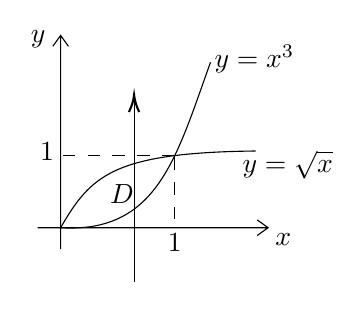
\begin{tikzpicture}[x=0.75pt,y=0.75pt,yscale=-.75,xscale=.75]
	 		\draw  (50,177.55) -- (198.1,177.55)(64.81,54) -- (64.81,191.27) (191.1,172.55) -- (198.1,177.55) -- (191.1,182.55) (59.81,61) -- (64.81,54) -- (69.81,61)  ;
	 		\draw    (64.81,177.55) .. controls (84.1,144.27) and (98.1,129.27) .. (190.1,128.27) ;
	 		\draw    (64.81,177.55) .. controls (127.1,181.27) and (139.1,132.27) .. (161.1,71.27) ;
	 		\draw    (112,212.27) -- (112,94.27) ;
	 		\draw [shift={(112,92.27)}, rotate = 90] [color={rgb, 255:red, 0; green, 0; blue, 0 }  ][line width=0.75]    (10.93,-3.29) .. controls (6.95,-1.4) and (3.31,-0.3) .. (0,0) .. controls (3.31,0.3) and (6.95,1.4) .. (10.93,3.29)   ;
	 		\draw  [dash pattern={on 4.5pt off 4.5pt}]  (138.1,132.27) -- (138.1,177.27) ;
	 		\draw  [dash pattern={on 4.5pt off 4.5pt}]  (138.1,131.27) -- (64.1,131.27) ;
	 		\draw (201,179.4) node [anchor=north west][inner sep=0.75pt]    {$x$};
	 		\draw (44,49.4) node [anchor=north west][inner sep=0.75pt]    {$y$};
	 		\draw (95,148.4) node [anchor=north west][inner sep=0.75pt]    {$D$};
	 		\draw (180,126.4) node [anchor=north west][inner sep=0.75pt]    {$y=\sqrt{x}$};
	 		\draw (162,58.4) node [anchor=north west][inner sep=0.75pt]    {$y=x^{3}$};
	 		\draw (132,179.4) node [anchor=north west][inner sep=0.75pt]    {$1$};
	 		\draw (50,121.4) node [anchor=north west][inner sep=0.75pt]    {$1$};
	 		\end{tikzpicture}
	 	\end{center}
	 	\[\begin{aligned}\iint_D4xy-y^3\ \d A=\int_0^1\int_{x^3}^{\sqrt{x}}4xy-y^3\ \d y\d x&=\int_0^1\qty[2xy^2-\dfrac{1}{4}y^4]_{x^3}^{\sqrt{x}}\ \d x\\&=\int_0^12x\qty(x-x^6)-\dfrac{1}{4}\qty(x^2-x^{12})\ \d x\\&=\int_0^12x^2-2x^7-\dfrac{1}{4}x^2+\dfrac{1}{4}x^{12}\ \d x\\&=\qty[\dfrac{2}{3}x^3-\dfrac{1}{4}x^8-\dfrac{1}{12}x^3+\dfrac{1}{52}x^{13}]_0^1\\&=\dfrac{2}{3}-\dfrac{1}{4}-\dfrac{1}{12}+\dfrac{1}{52}=\dfrac{55}{156}.\end{aligned}\]
	 \end{sol}
\end{eg}



\end{document}